\chapter{2D Multi-view Discriminant Analysis}
\label{ch:2DMvDA}
\noindent {\textbf{\huge T}}his chapter presents a batch classification method for 2D multi-view data. Using 1D methods to train on naturally 2D data leads to the loss of valuable spatial information. Also, the vectorization leads to larger scatter matrices. The use of 2D methods for 2D data preserves spatial information and eliminates the need for vectorization. Hence, we propose a 2D batch method for multi-view data to train a classification model in less time and memory.

The proposed method, 2D Multi-view Discriminant Analysis (2DMvDA), is designed to serve as a basis for an incremental-decremental 2D method presented in Chapter \ref{ch:2DMvIDDA}. 2DMvDA has a very straightforward formulation. However, the main idea is to introduce 2D methods to the realm of multi-view learning. It utilizes the matrix form of images to preserve spatial information and reduce the size of scatter matrices for better and faster performance. 2DMvDA also eliminates the need for feature extraction in preprocessing stage.

We present the formulations of 2DMvDA followed by the experimental setup and results. We conclude this chapter by summarizing the features of 2DMvDA.









\section{Methodology}
\label{sec:2DMvDA_Algo}
2DMvDA works on the same principle of discriminant analysis as MvDA. The within-class scatter and the between-class scatter are defined as follows,

\begin{equation}
\label{eqn:2DMvDA_Sw}
\textbf{S}_W = \sum_{i=1}^{c} \sum_{j=1}^{v} \sum_{k=1}^{n_{ij}} \left ( \textbf{Y}_{ijk} - \textbf{M}_{i} \right ) \left ( \textbf{Y}_{ijk} - \textbf{M}_{i} \right )^T
\end{equation}

\begin{equation}
\label{eqn:2DMvDA_Sb}
\textbf{S}_B = \sum_{i=1}^{c} n_i \left ( \textbf{M}_{i} - \textbf{M} \right ) \left ( \textbf{M}_{i} - \textbf{M} \right )^T
\end{equation}

Note that these equations are similar to those of MvDA. However, here we compute the scatter matrices using 2D data matrices in contrast to 1D feature vectors used by MvDA. Eq. \ref{eqn:2DMvDA_Sw} and Eq. \ref{eqn:2DMvDA_Sb} are in terms of the data samples in projected space ($\textbf{Y}_{ijk}$). We reformulate these equations in terms of the original data samples ($\textbf{X}_{ijk}$). The reformulated within-class scatter is given as,


\begin{equation}
\label{eqn:2DMvDA_Sjr}
\textbf{S}_{jr} = \left\{\begin{matrix*}[l]
\sum_{i=1}^{c} \left ( \sum_{k=1}^{n_{ij}} \textbf{X}_{ijk }\textbf{X}_{ijk}^T - \frac{n_{ij} n_{ij}}{n_i} \textbf{M}_{ij}^{(\textbf{X})} \textbf{M}_{ij}^{(\textbf{X})T} \right ) & \cdots j=r \\ 
-\sum_{i=1}^{c} \frac{n_{ij} n_{ir}}{n_i} \textbf{M}_{ij}^{(\textbf{X})} \textbf{M}_{ir}^{(\textbf{X})T} & \cdots j\neq r 
\end{matrix*}\right.
\end{equation}

\noindent
Here, $\textbf{S}_{jr}$ is computed using the 2D matrices in the original space. The derivation for Eq. \ref{eqn:2DMvDA_Sjr} is given in Appendix-E.%\ref{proof:2DMvDA_Sjr}.

\noindent
The reformulated equation for between-class scatter is given as,


\begin{equation}
\label{eqn:2DMvDA_Djr}
\begin{split}
\textbf{D}_{jr} = \sum_{i=1}^{c} \frac{n_{ij} \; n_{ir}}{n_i} \; \textbf{M}_{ij}^{(\textbf{X})} \; \textbf{M}_{ir}^{(\textbf{X})T} - \frac{1}{n} & \left ( \sum_{i=1}^{c} n_{ij} \; \textbf{M}_{ij}^{(\textbf{X})} \right )\left ( \sum_{i=1}^{c} n_{ir} \; \textbf{M}_{ir}^{(\textbf{X})} \right )^T
\end{split}
\end{equation}

Here, $\textbf{D}_{jr}$ is computed using the 2D matrices in the original space. The derivation for Eq. \ref{eqn:2DMvDA_Djr} is given in Appendix-A.%\ref{proof:Djr}.

We convert Eq. \ref{eqn:Lit_MvDA_Wopt} into a ratio trace function so that it can be solved as a generalized eigenvalue problem. The reformulated optimal function is,

\begin{equation}
\label{eqn:2DMvDA_WoptRT}
\textbf{W}^{opt} = \left( \textbf{W}_1^{opt}, \cdots, \textbf{W}_v^{opt} \right) = \underset{(\textbf{W}_1,\textbf{W}_2,\cdots,\textbf{W}_v)}{argmax}Tr\left ( \frac{\textbf{W}^T \textbf{D} \textbf{W}}{\textbf{W}^T \textbf{S} \textbf{W}} \right )
\end{equation}

\noindent
The above equation can now be solved using the Generalized eigenvalue decomposition method as,

\begin{equation}
\label{eqn:2DMvDA_GEP}
\textbf{D} \textbf{W}^{opt}=\lambda \textbf{S} \textbf{W}^{opt}
\end{equation}

We then form $\textbf{W}^{opt}$, a matrix of optimal projection vectors, by selecting the eigenvectors corresponding to the first $d$ largest eigenvalues of $\textbf{S}^{-1} \textbf{D}$. This projection matrix is then used to project the test samples onto a common discriminant subspace. The projection of a test sample of size $p_j \times q$, will be of size $d \times q$ in the common discriminant subspace.










\section{Experiments and Results}
\label{sec:2DMvDA_Expt}

\subsection{Experimental Setup}
\label{subs:2DMvDA_Expt_Setup}
MvDA, being a 1D method, needs the training data in vectorized format. However, due to the large images in these datasets, MvDA needed more than 100 Terabytes of processing memory. Hence, we used rescaled versions of datasets to train the models $\phi_A$, $\phi_B$ and $\phi_C$ using 2DMvDA, 2DLDA, and MvDA, respectively.

In another set of experiments, we used original versions of the datasets mentioned above to show the full strength of 2DMvDA. This time, we trained the models only on 2DMvDA and 2DLDA. We have divided each dataset into two parts for both sets of experiments. 80\% of the total data samples are used to train the models. The remaining 20\% data samples are used as a test set.

To compare the three methods, we record the time and memory required by these methods to train classification models. Also, to compare the classification accuracy of these models, we extract 10 sets of eigenvectors corresponding to first $d$ largest eigenvalues where, $d = \left \{ i*2|i=1, \cdots, 10 \right \}$. These eigenvectors form the projection matrix $\textbf{W}^{opt}$ and are used to project each test data sample ($\textbf{Y}^{Test}$) onto the common discriminant subspace. The methodology for classification is the same as that used for MvIDA.










\subsection{Results}
\label{subs:2DMvDA_Res}
This section presents the results of experiments designed in order to answer the research questions posed in chapter \ref{ch:Intro}.



\subsubsection{A. Classification Accuracy}
\label{ssubs:2DMvDA_Acc}
\begin{figure}[t]
\centering
  \begin{subfigure}[h]{0.48\textwidth}
    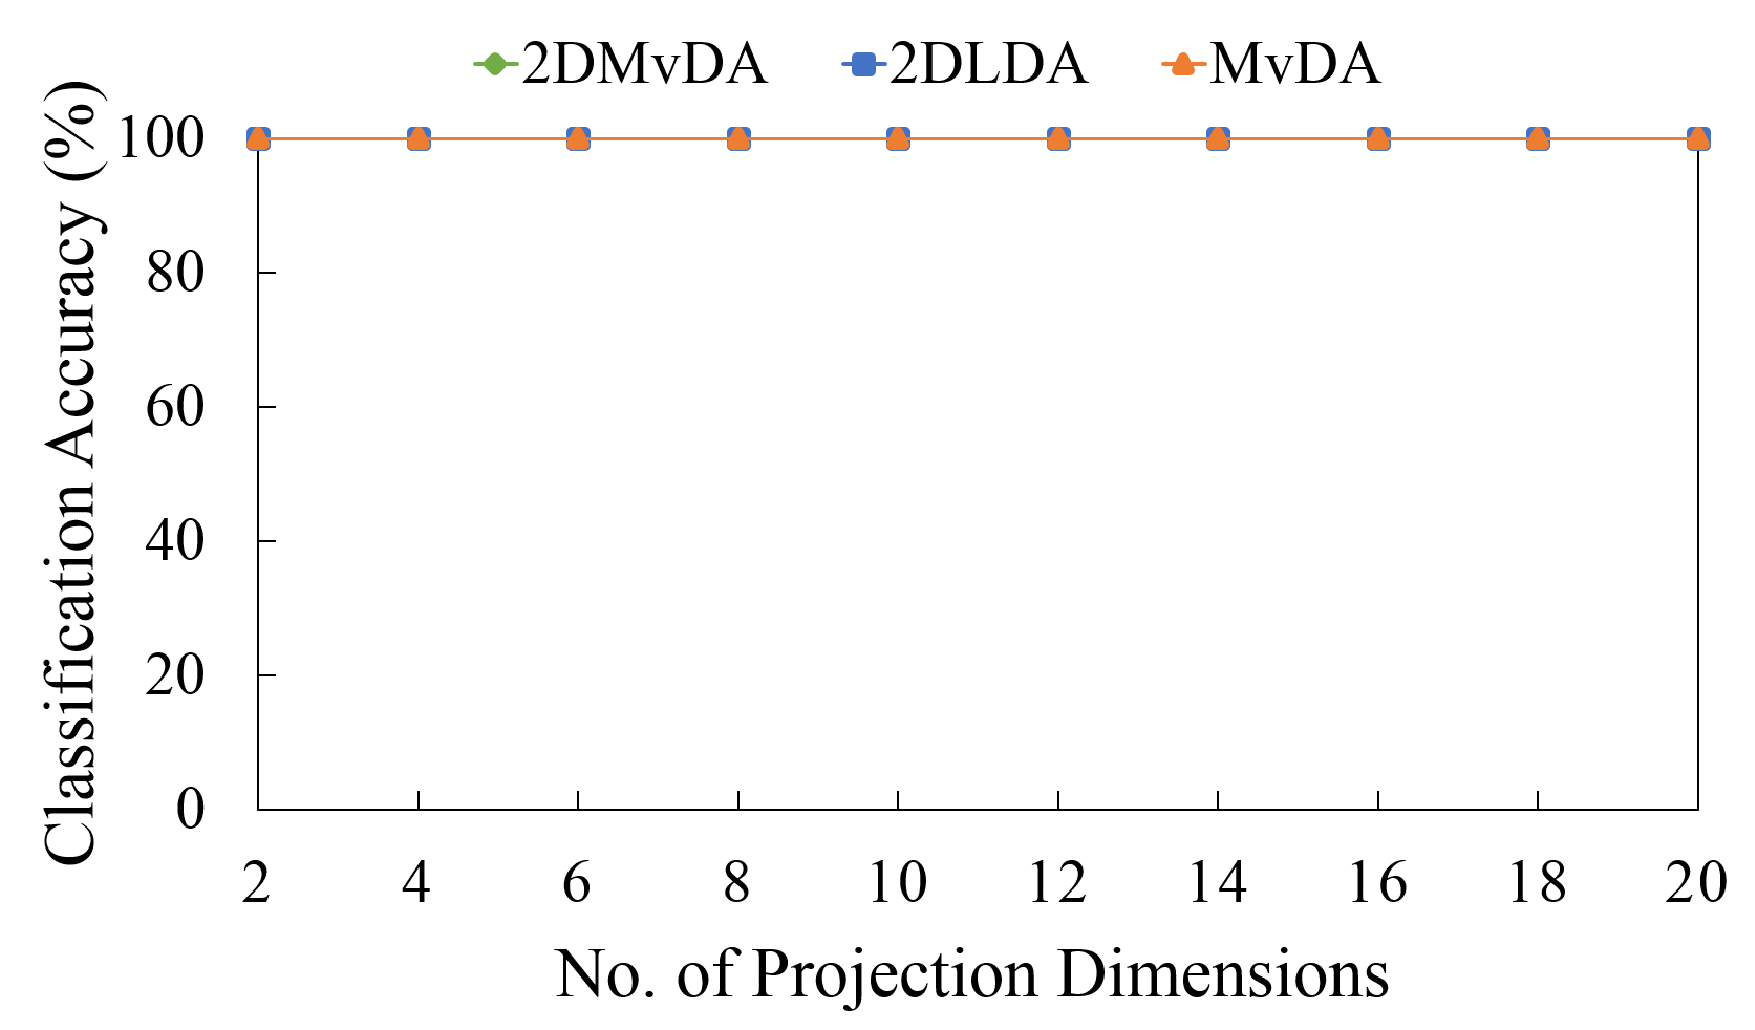
\includegraphics[width=\textwidth]{Figures/2DMvDA/Fig1.pdf}
    \caption{IMPART face dataset}
  \end{subfigure}
  \begin{subfigure}[h]{0.48\textwidth}
    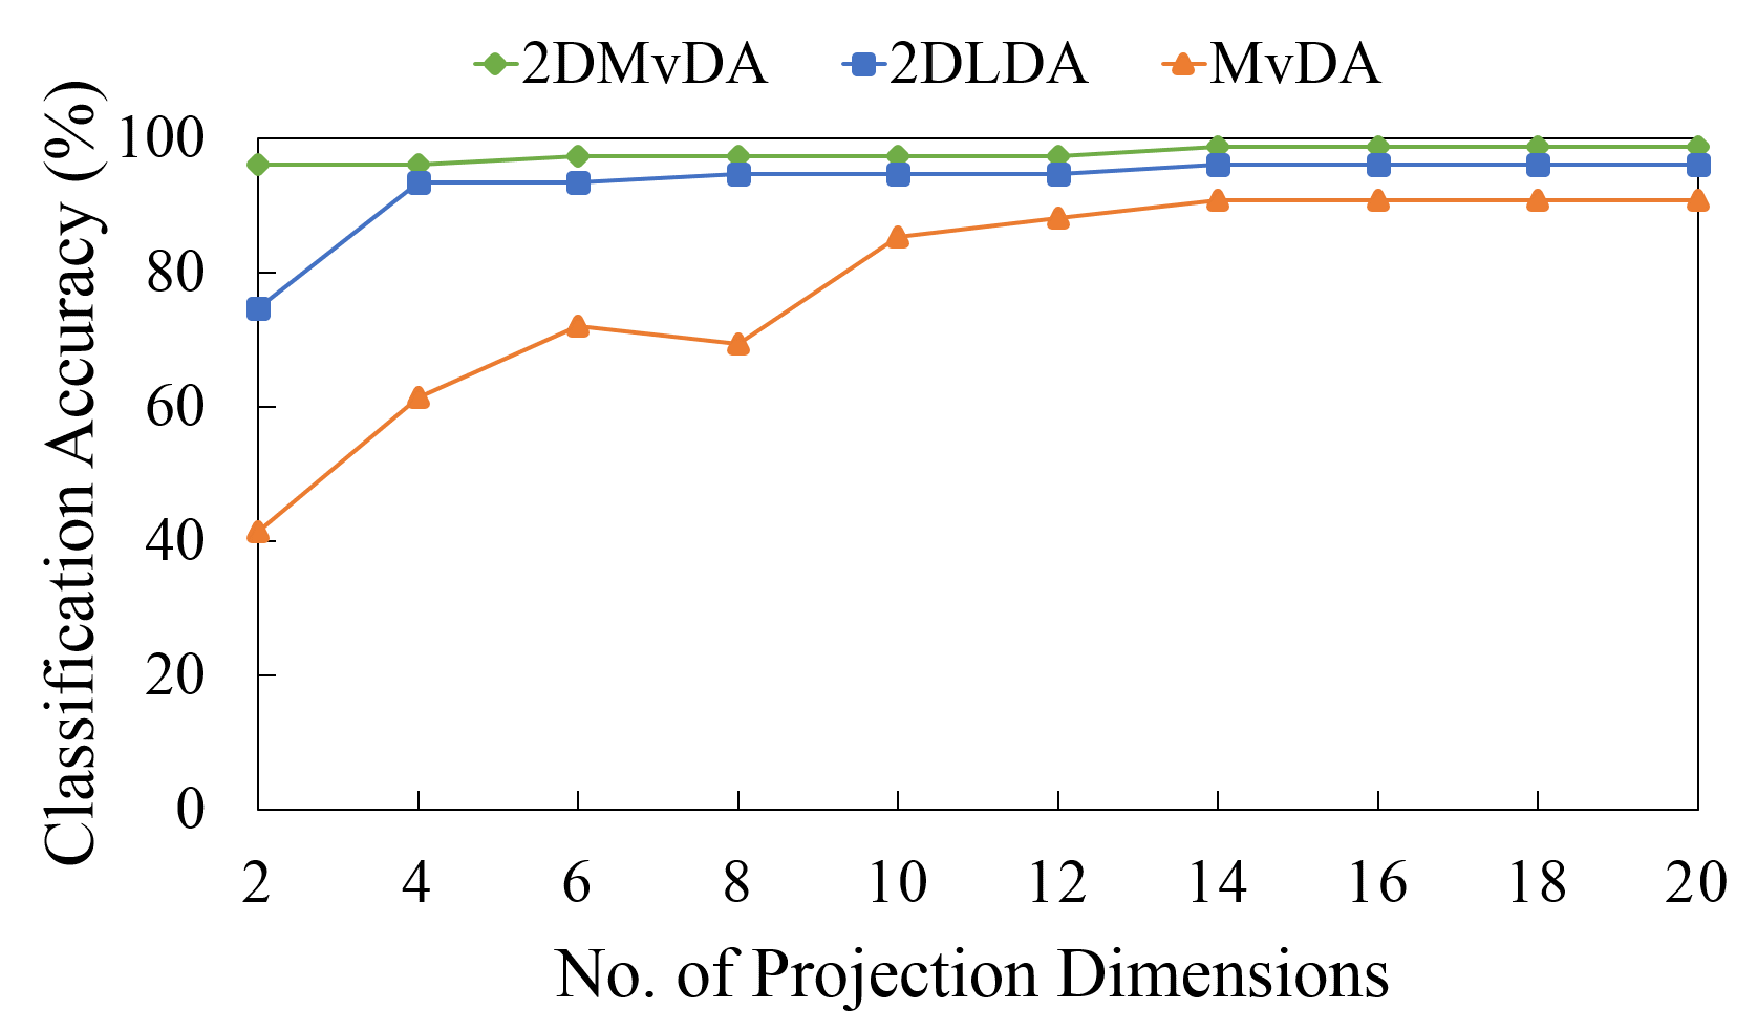
\includegraphics[width=\textwidth]{Figures/2DMvDA/Fig2.pdf}
    \caption{MSSpoof dataset}
  \end{subfigure}
  
  \begin{subfigure}[h]{0.48\textwidth}
    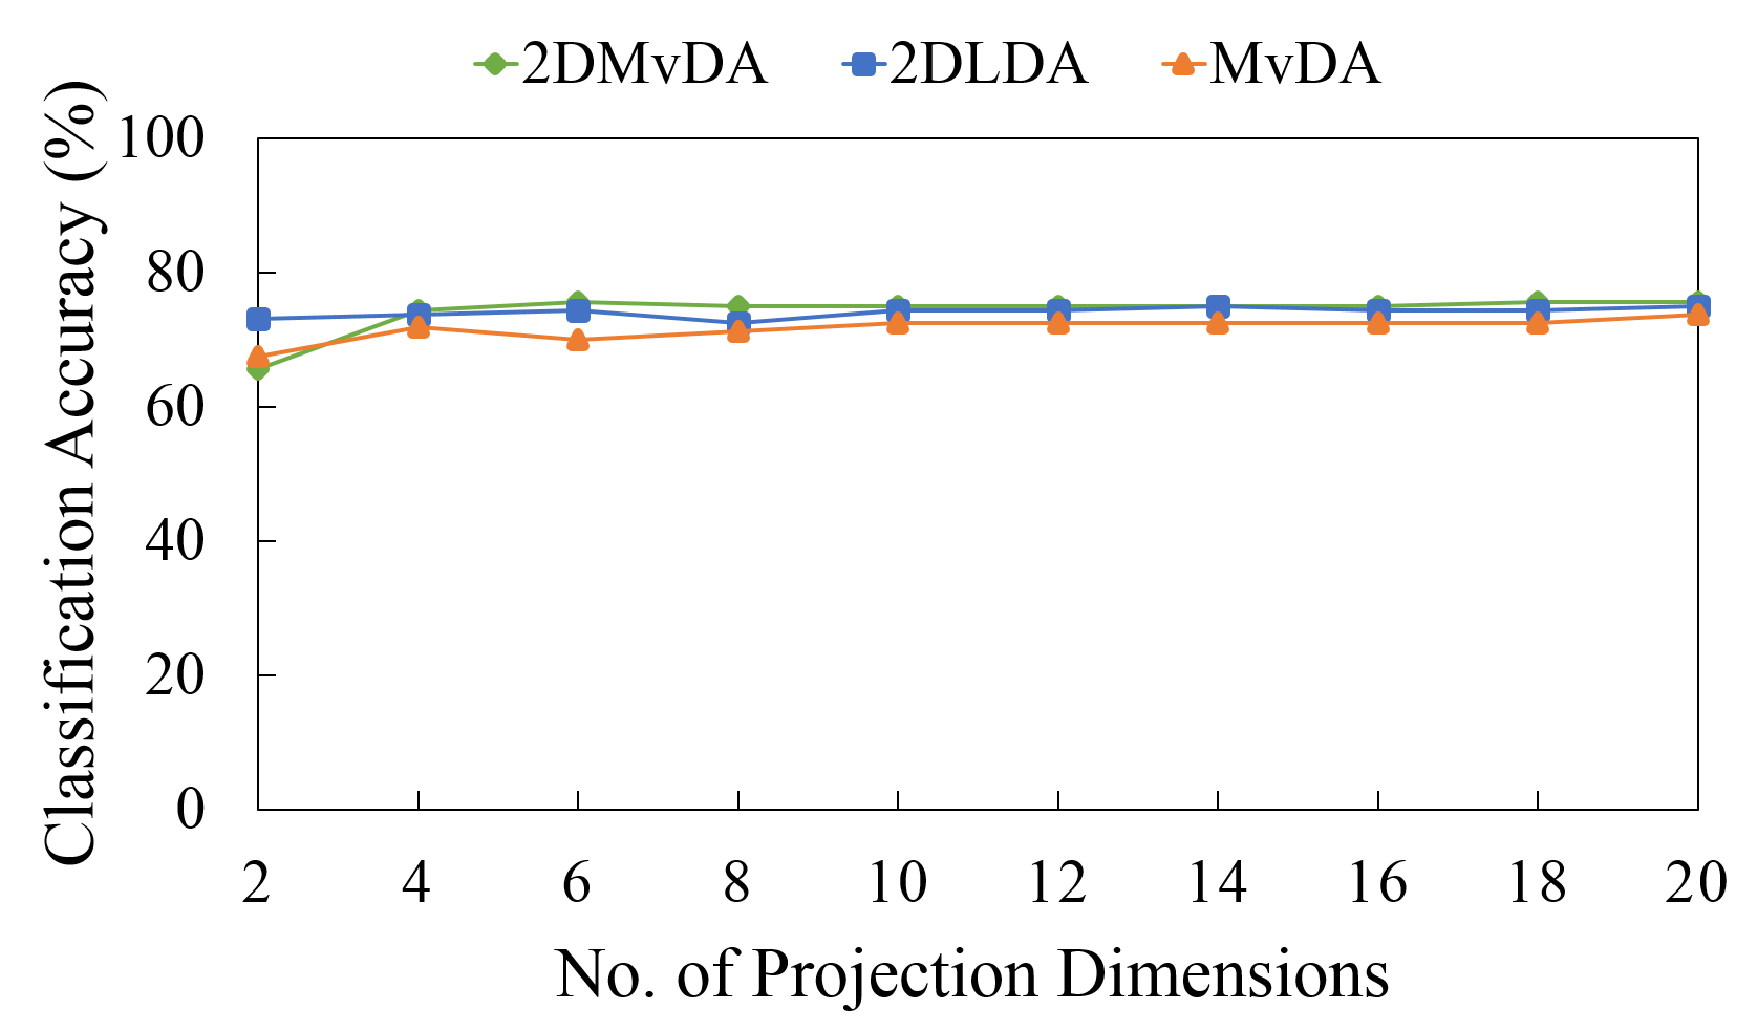
\includegraphics[width=\textwidth]{Figures/2DMvDA/Fig3.pdf}
    \caption{Stereo face dataset}
  \end{subfigure}
  \begin{subfigure}[h]{0.48\textwidth}
    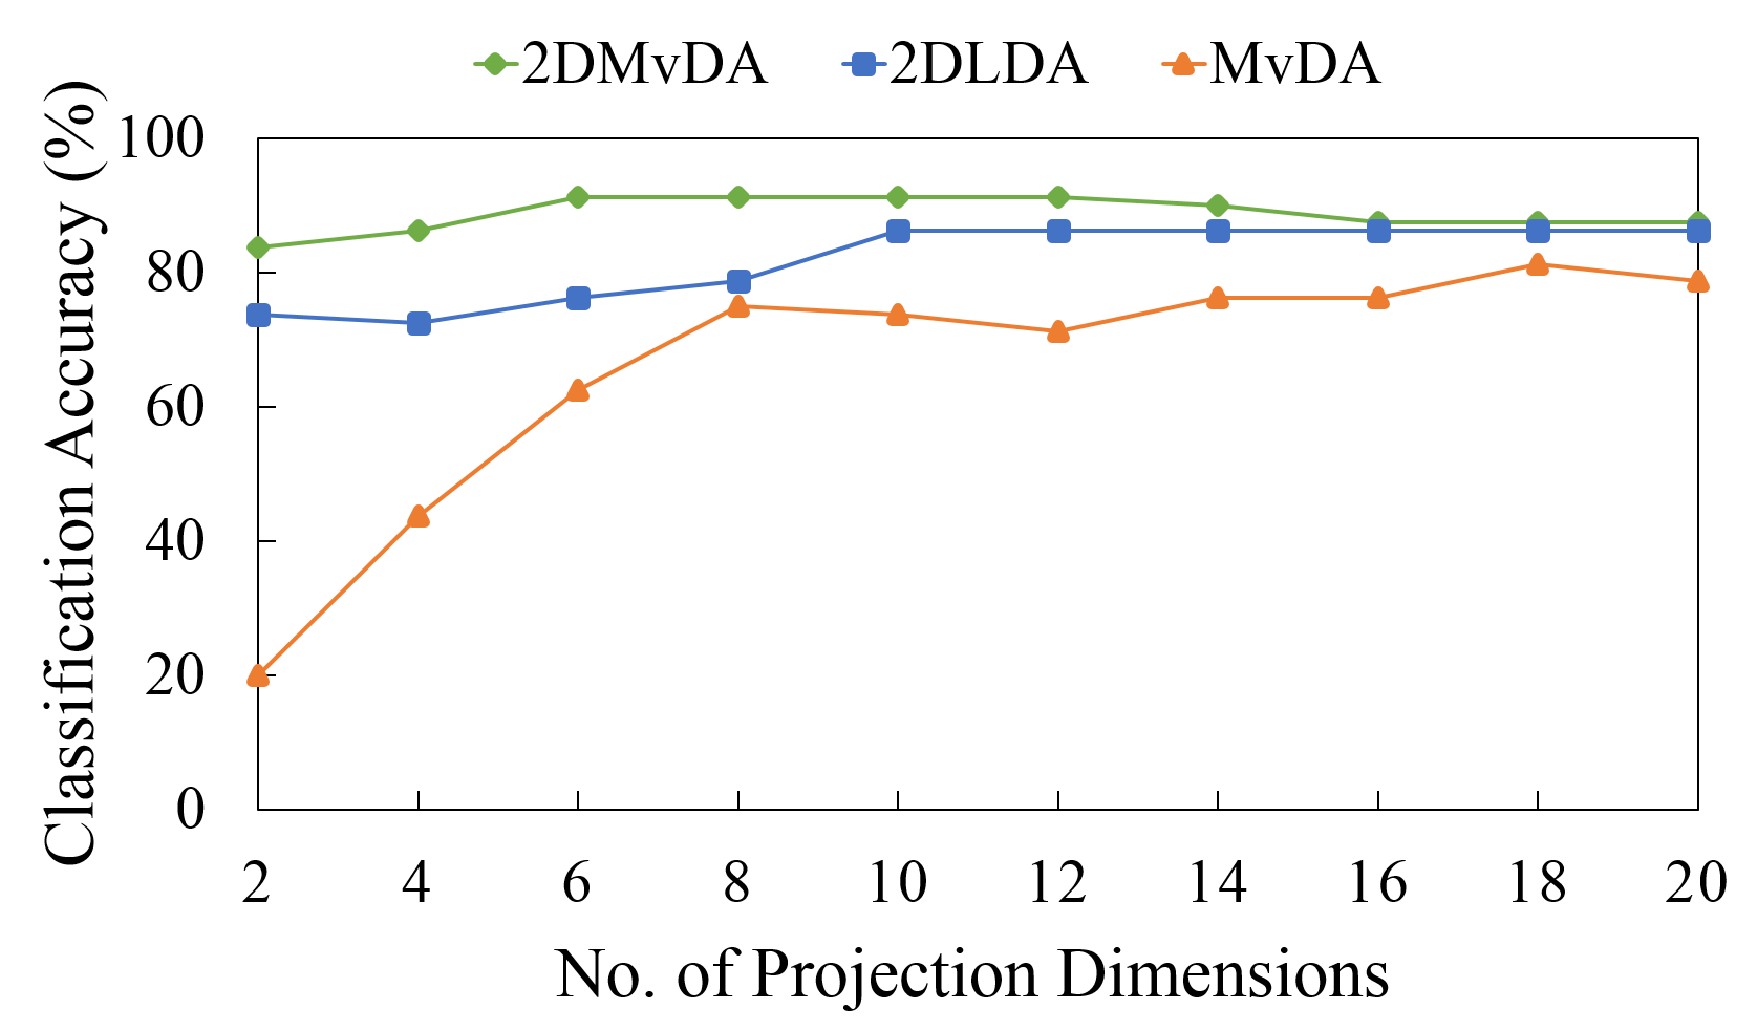
\includegraphics[width=\textwidth]{Figures/2DMvDA/Fig4.pdf}
    \caption{ORL dataset}
  \end{subfigure}
  
\caption{Classification accuracy vs. number of projection dimensions (On rescaled datasets)}
\label{fig:2DMvDA_Res_Acc}
\end{figure}

\begin{itemize}
\item \textbf{RQ1 :}
Can a 2D multi-view method build a better classification model than a 1D multi-view method or a 2D single-view method?

\item \textbf{Experiment :}
Record classification accuracy of the methods by varying the no. of projection dimensions $d = \left \{ i*2|i=1, \cdots, 10 \right \}$.

\item \textbf{Discussion :}
Fig. \ref{fig:2DMvDA_Res_Acc} compares the accuracies of these three methods. We see that the classification accuracy of 2DMvDA is better than or the same as that of the other two methods. 2DMvDA performs much better than MvDA even in lower-dimensional space as the former extracts the 2D features that provide more information than the 1D features. We also see that 2DMvDA performs at par or better than 2DLDA, despite both being 2D methods. This is because 2DLDA considers all the views as one, depriving itself of the discriminatory information that 2DMvDA gains by processing the views separately. This proves the benefits of using two-dimensional representation and multiple views.

We have plotted the classification results of these three methods on the MSSpoof dataset using t-SNE. Fig. \ref{fig:2DMvDA_Res_VisRS} shows the results. Here, the training data samples from different classes are shown in different colors. The correctly classified test data samples are denoted with black squares, and those classified incorrectly are denoted with red triangles. We see that the subspace constructed by 2DMvDA and 2DLDA is better at discriminating between different classes than MvDA. This leads to the better classification accuracy of 2D methods. MvDA performs poorly as it does not take spatial information into account.
\end{itemize}

\begin{figure}[t]
\centering
  \begin{subfigure}[h]{0.45\textwidth}
    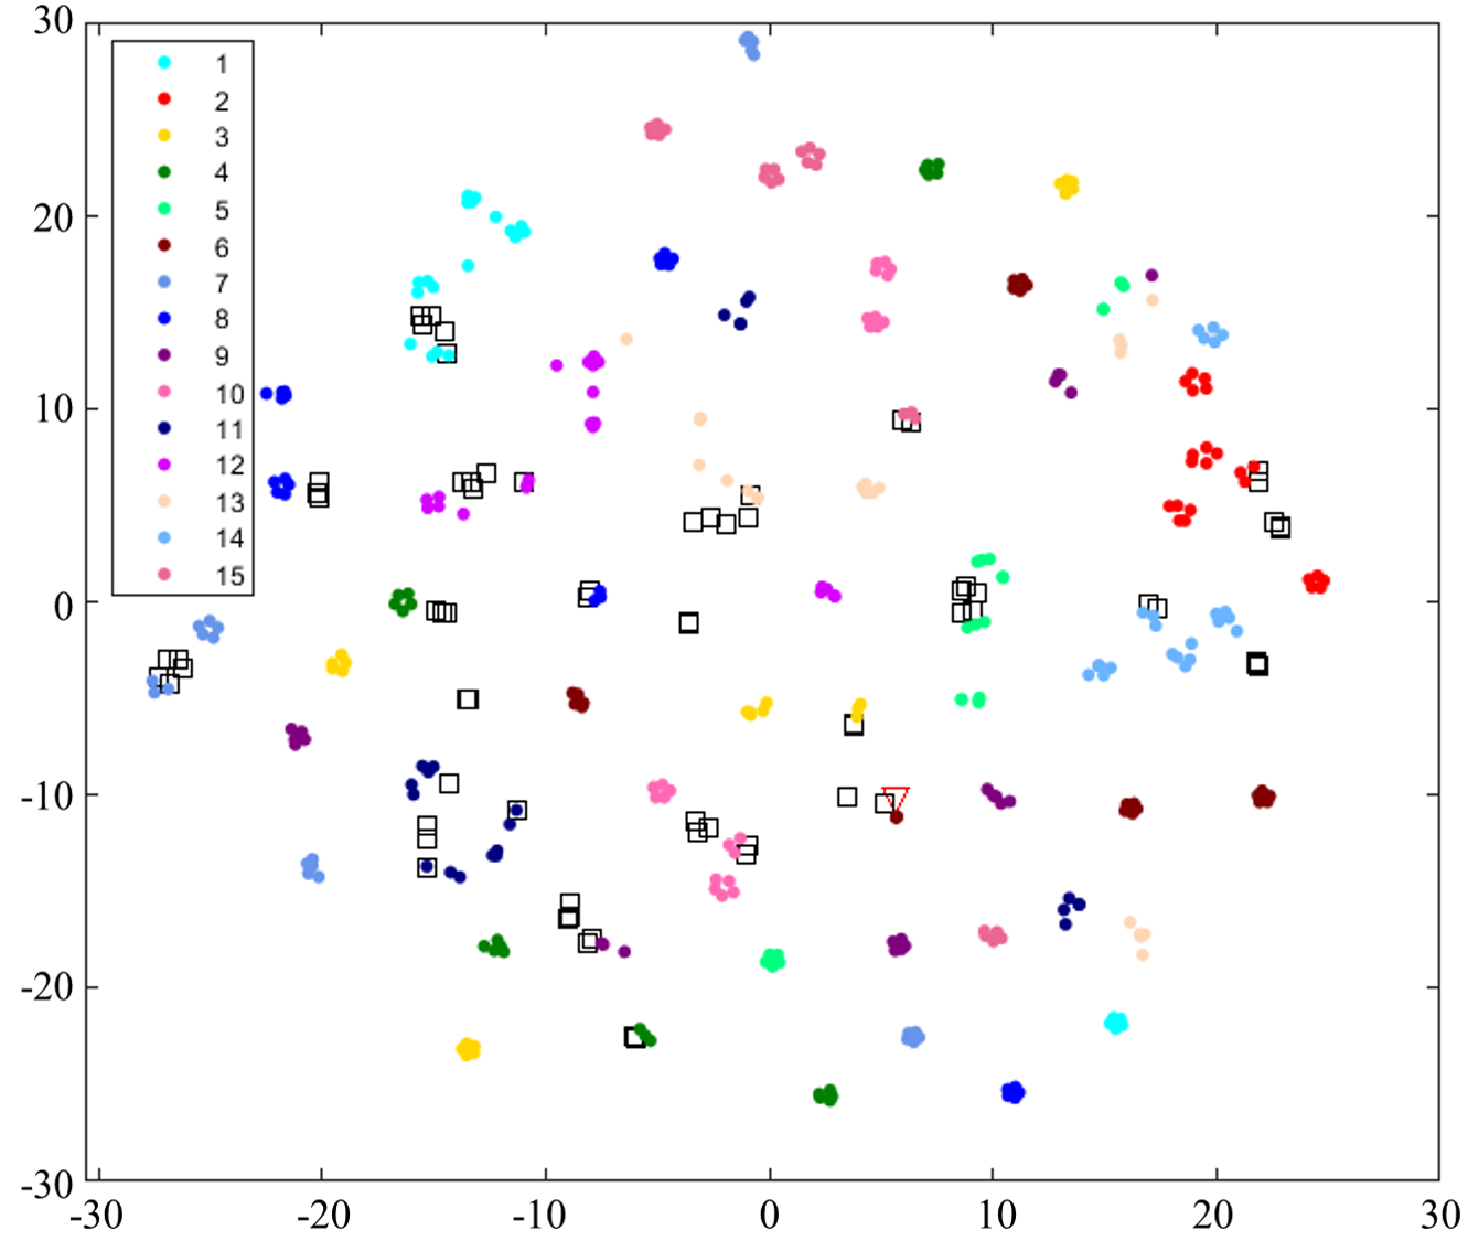
\includegraphics[width=\textwidth]{Figures/2DMvDA/Fig5.pdf}
    \caption{2DMvDA}
  \end{subfigure}

  \begin{subfigure}[h]{0.45\textwidth}
    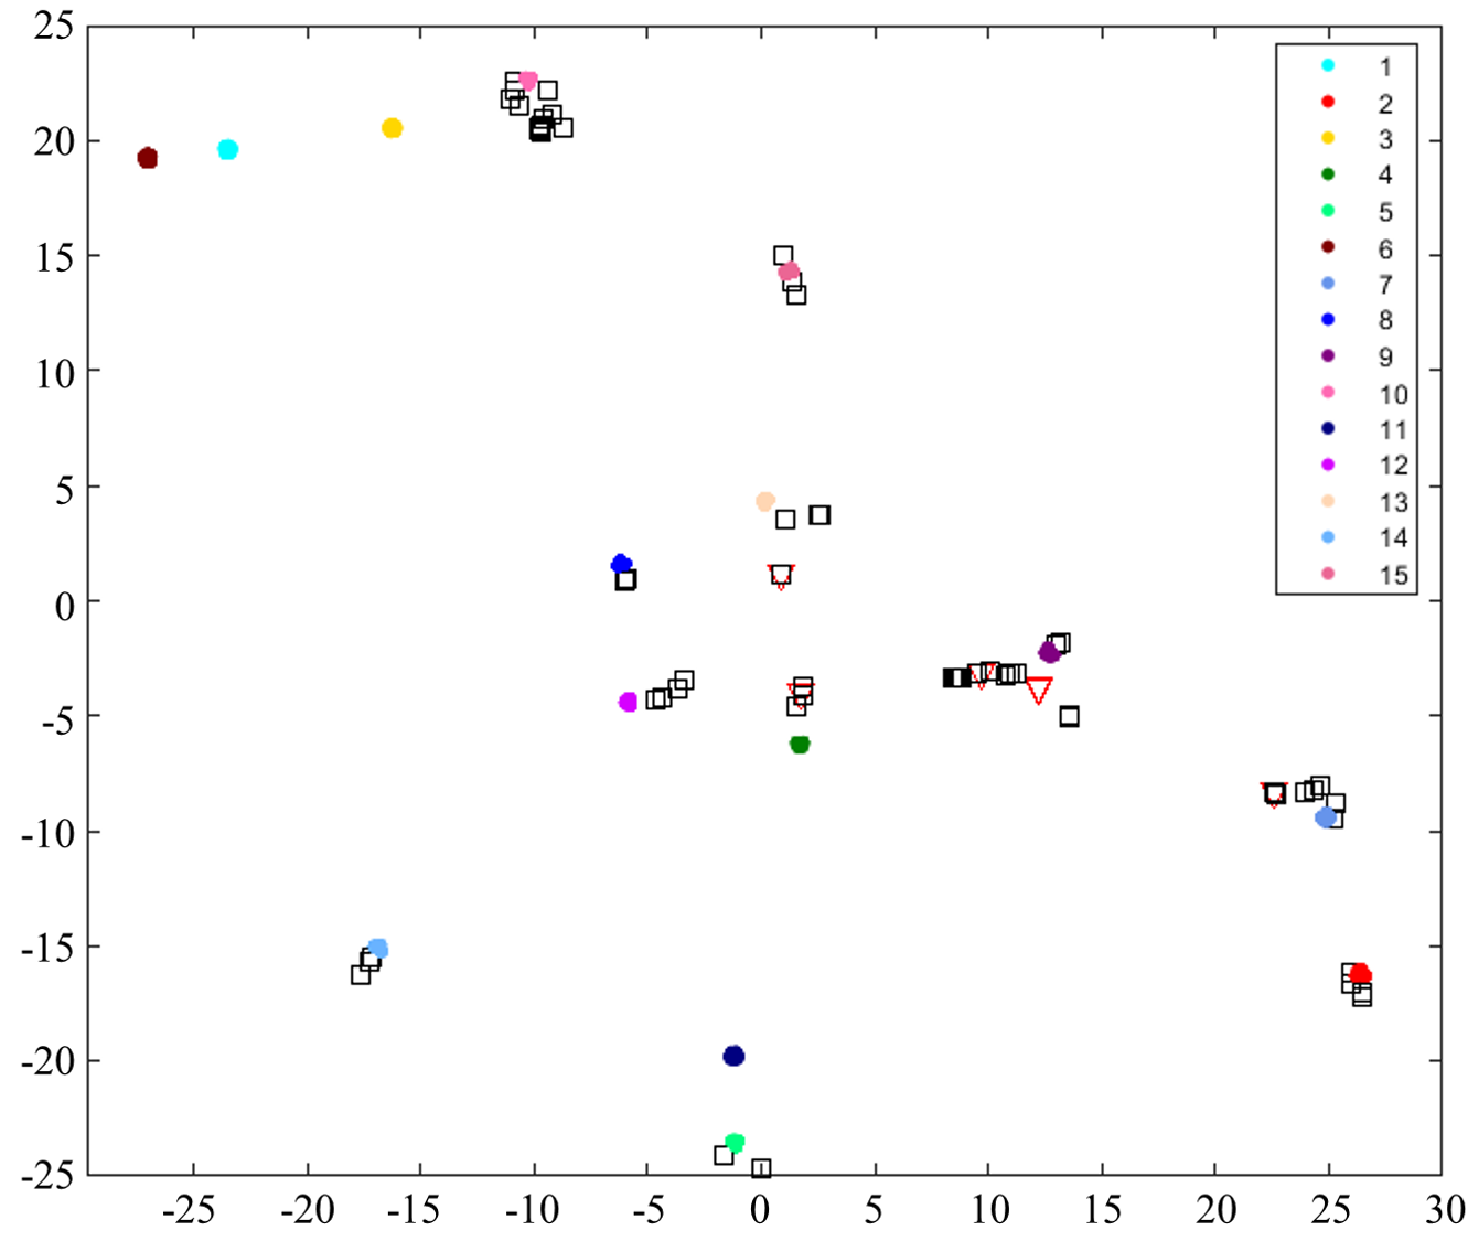
\includegraphics[width=\textwidth]{Figures/2DMvDA/Fig6.pdf}
    \caption{MvDA}
  \end{subfigure}  
  \begin{subfigure}[h]{0.45\textwidth}
    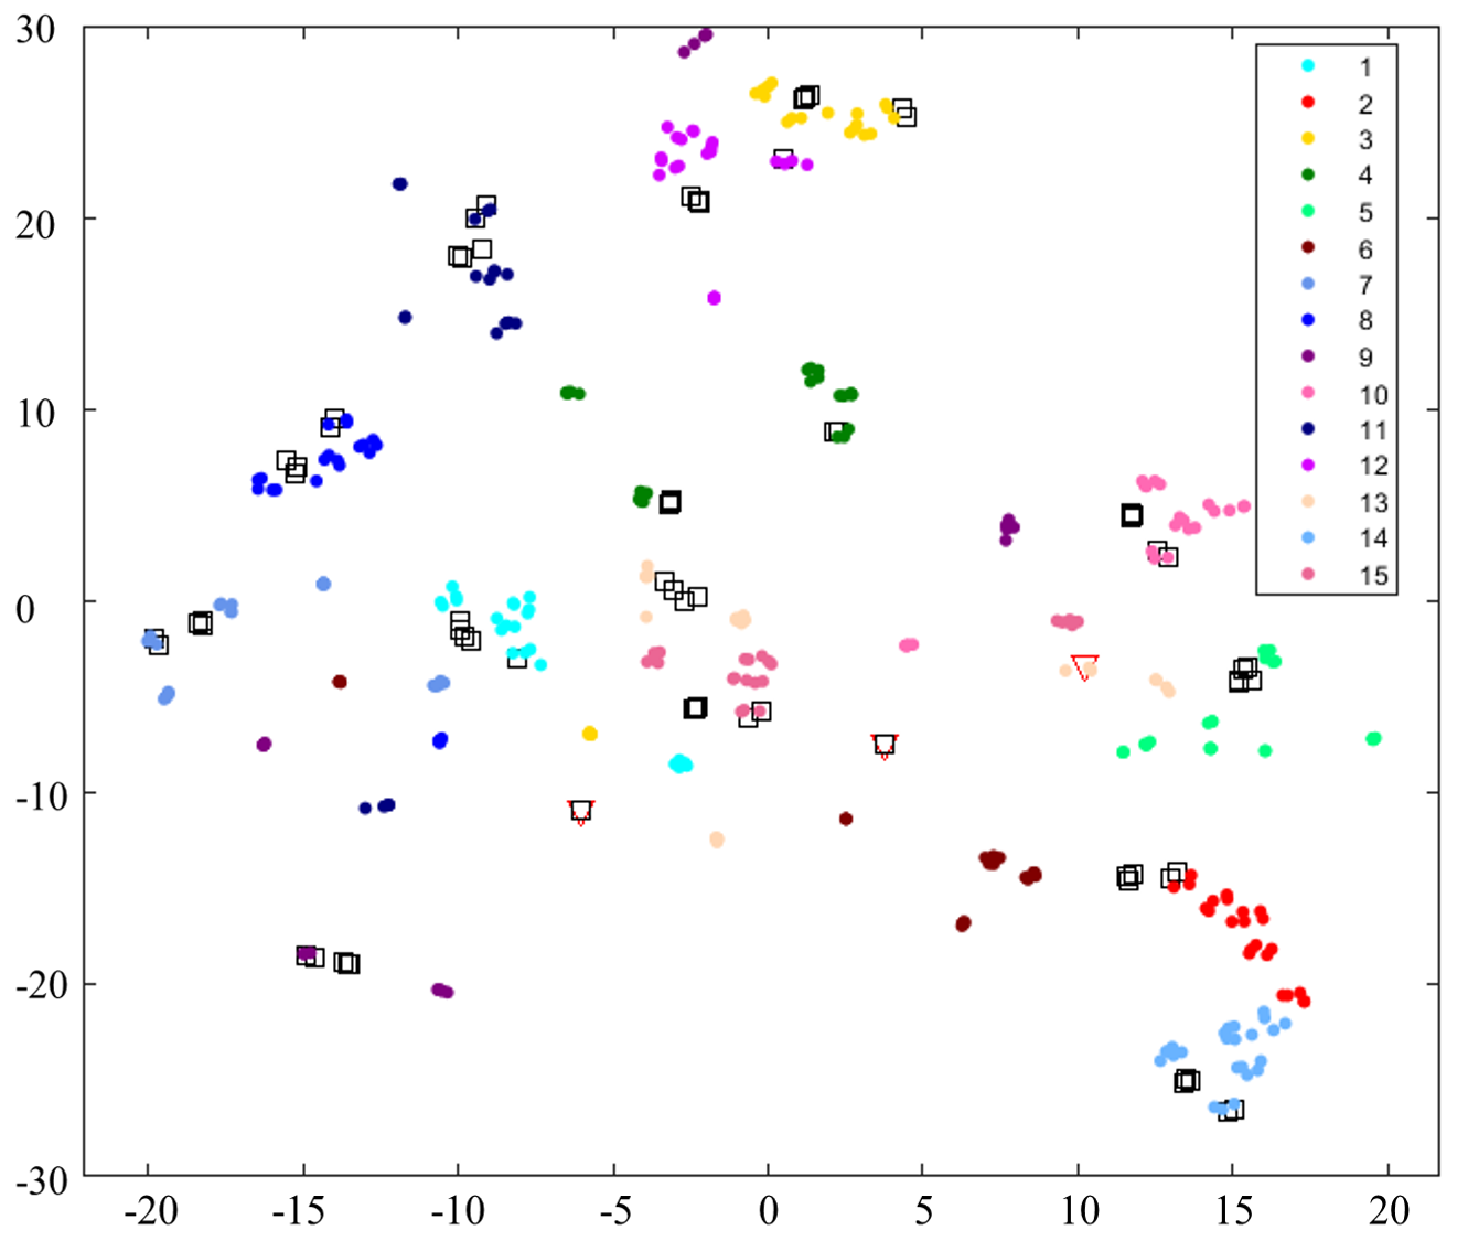
\includegraphics[width=\textwidth]{Figures/2DMvDA/Fig7.pdf}
    \caption{2DLDA}
  \end{subfigure}
  
\caption{Visualization of Classification on MSSpoof Dataset: (i) Training data samples are denoted with different colors for each class. (ii) Correctly classified test samples are denoted with hollow black squares. (iii) Misclassified test samples are denoted with hollow red triangles.}
\label{fig:2DMvDA_Res_VisRS}
\end{figure}











\subsubsection{Training Time}
\label{ssubs:2DMvDA_Time}
\begin{itemize}
\item \textbf{RQ2 :}
Can the use of 2D matrices reduce training time?

\item \textbf{Experiment :}
Record training time of (i) all three methods on the rescaled datasets and (ii) 2DMvDA and 2DLDA on the original datasets.

\item \textbf{Discussion :}
Fig. \ref{fig:2DMvDA_Res_TimeRS} shows the records of training time of each method on the rescaled versions of all four datasets. The suffix (RS) represents the rescaled versions of the datasets. Note that the scale on the y-axis of 2DMvDA and 2DLDA is much smaller than that of MvDA. We see that the 2DMvDA requires less than a second to train the model, whereas the 1D method -MvDA- has much greater time requirements. The records of average training time on the original versions of the datasets using 2DMvDA and 2DLDA are presented in Fig. \ref{fig:2DMvDA_Res_TimeRS}.

The records of average training time of 2DMvDA and 2DLDA on original datasets are presented in Fig. \ref{fig:2DMvDA_Res_TimeOrig}. We see that 2DMvDA trains the model in 30\% to 70\% of the training time of 2DLDA. The experiments using MvDA could not be performed due to the larger memory requirements of this 1D method. However, by linearly extrapolating the time requirements on the rescaled dataset, we say that MvDA would need a little over 21 days to train on the original version of the IMPART dataset. 2DMvDA, on the other hand, needs only 3 minutes on the same dataset.
\end{itemize}

\begin{figure}[t]
	\centering
  \begin{subfigure}[h]{0.48\textwidth}
    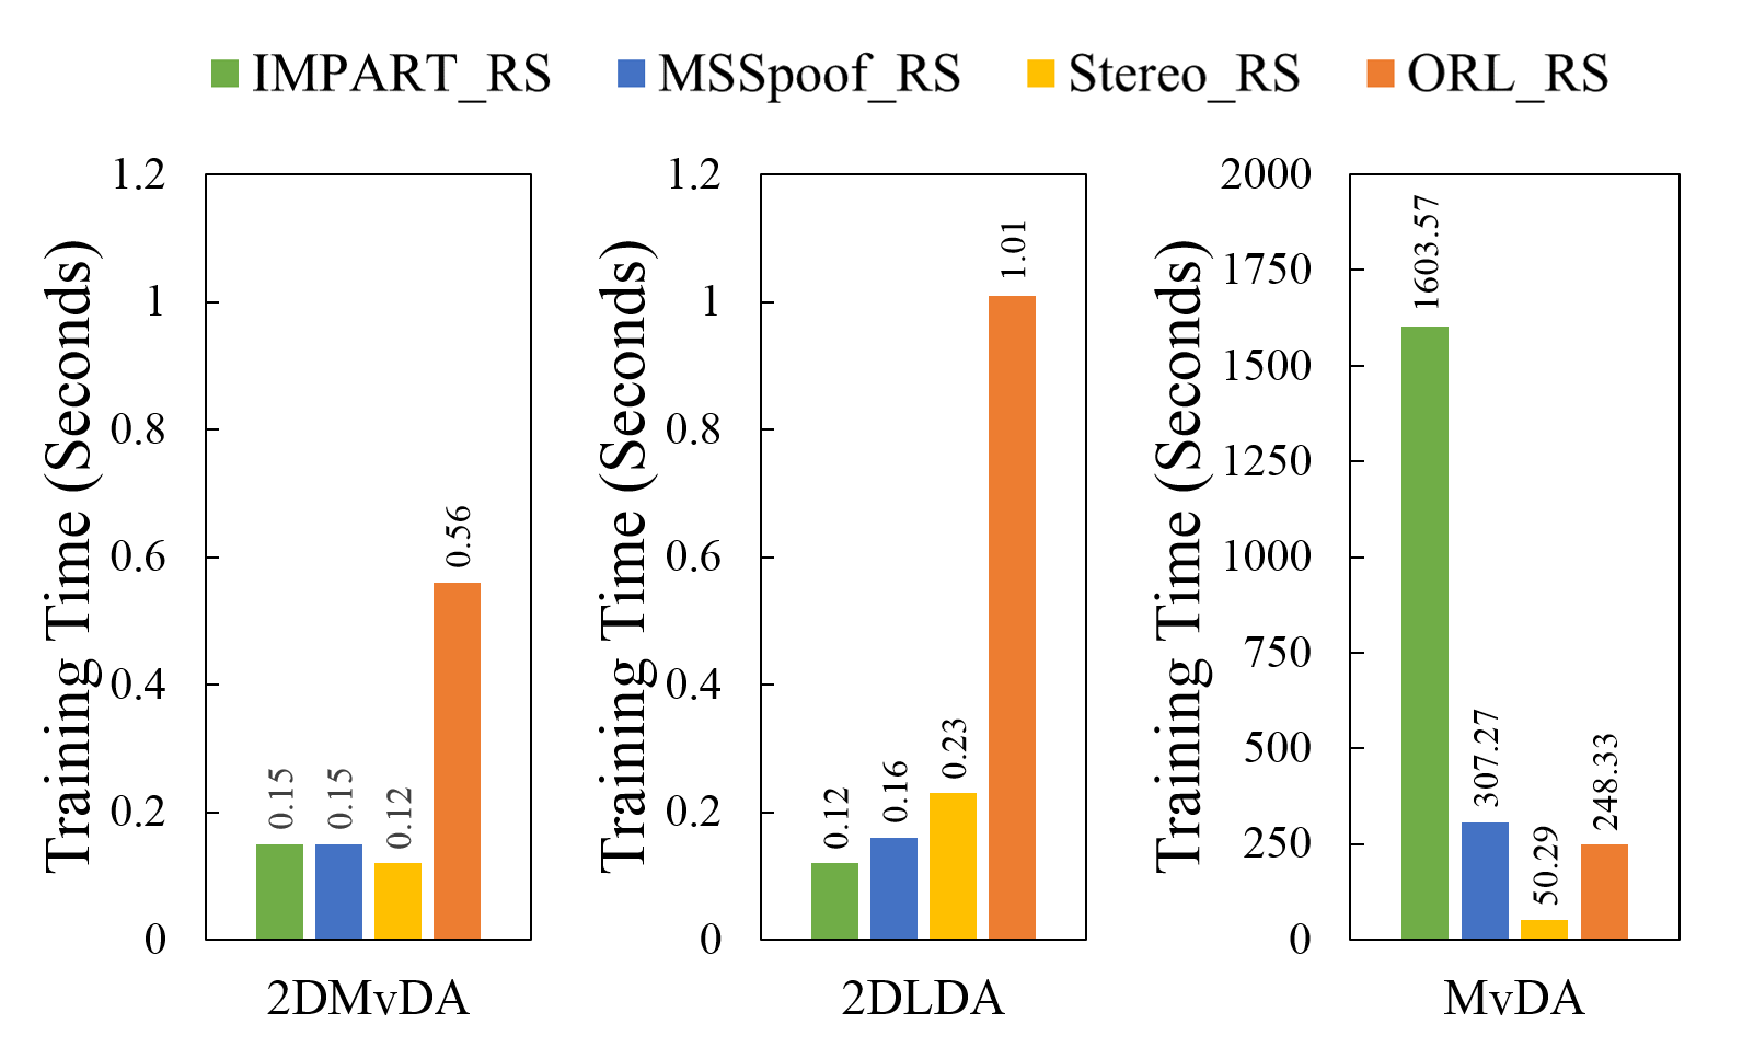
\includegraphics[width=\textwidth]{Figures/2DMvDA/Fig8.pdf}
    \caption{On rescaled datasets}
	\label{fig:2DMvDA_Res_TimeRS}
  \end{subfigure}
  \begin{subfigure}[h]{0.48\textwidth}
    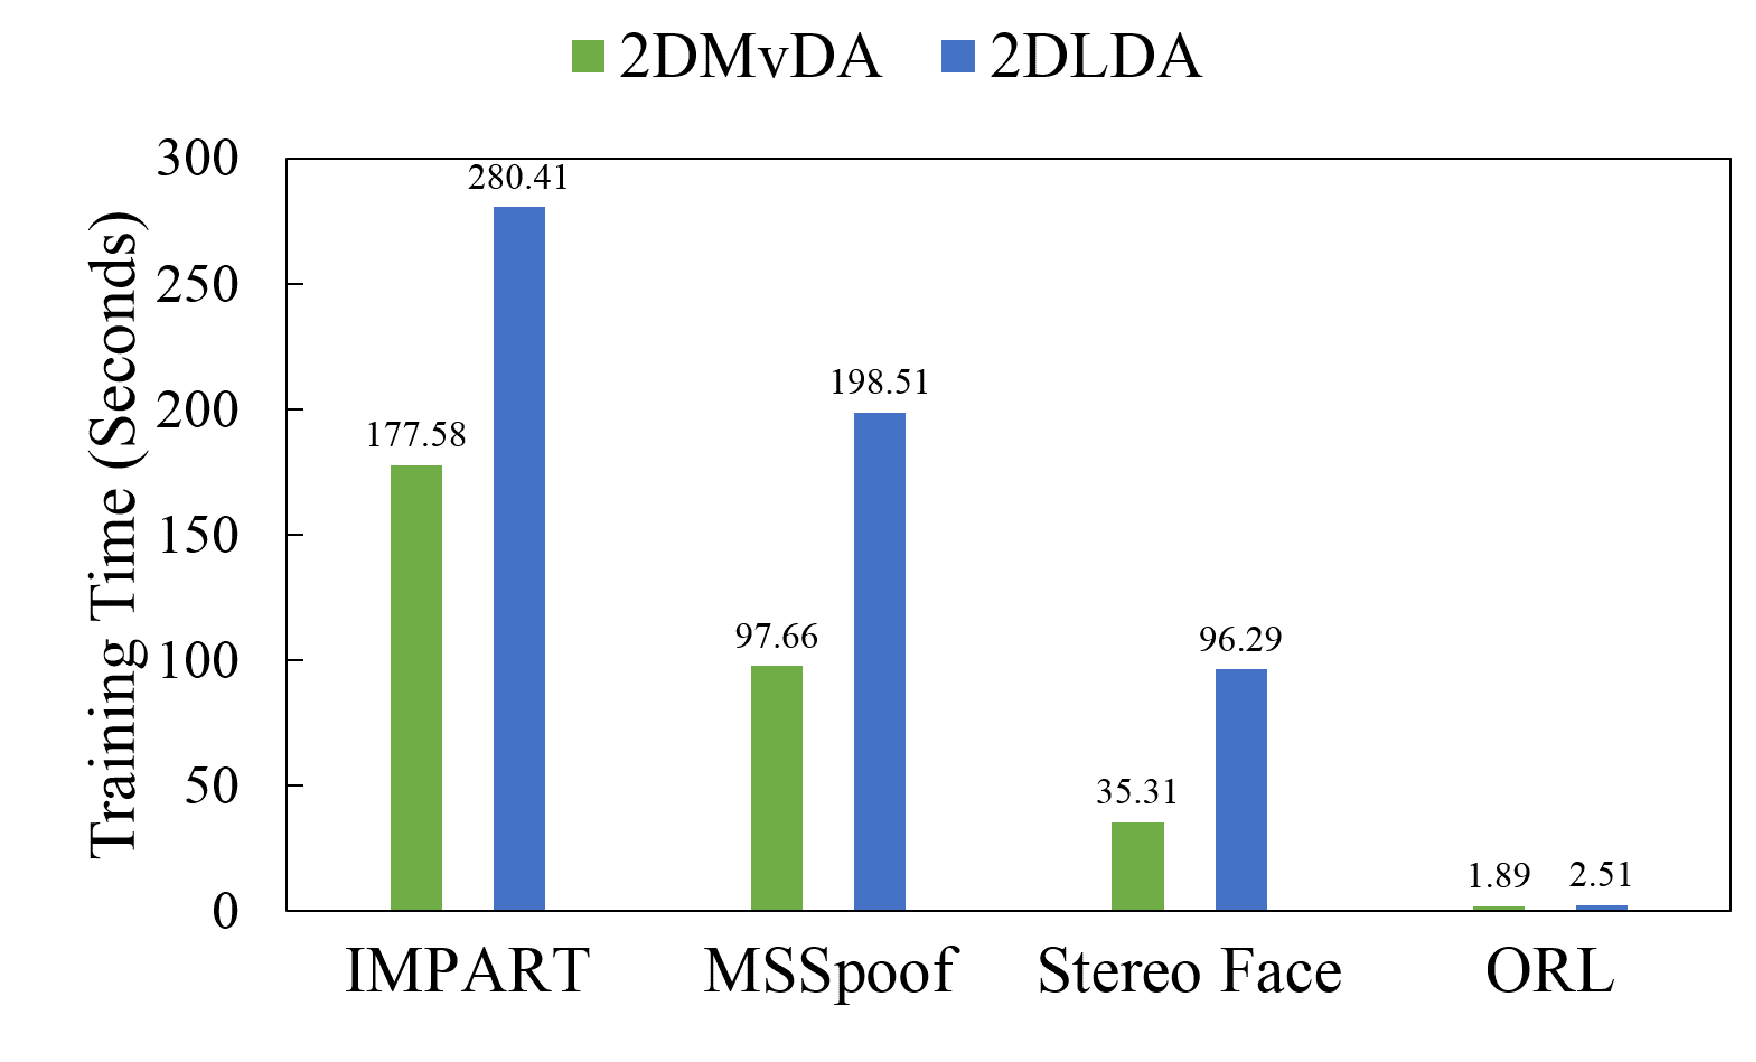
\includegraphics[width=\textwidth]{Figures/2DMvDA/Fig9.pdf}
    \caption{On original datasets}
	\label{fig:2DMvDA_Res_TimeOrig}
  \end{subfigure}
\caption{Comparison of training time}
\label{fig:2DMvDA_Res_Time}
\end{figure}












\begin{figure}[t]
	\centering
  \begin{subfigure}[h]{0.48\textwidth}
    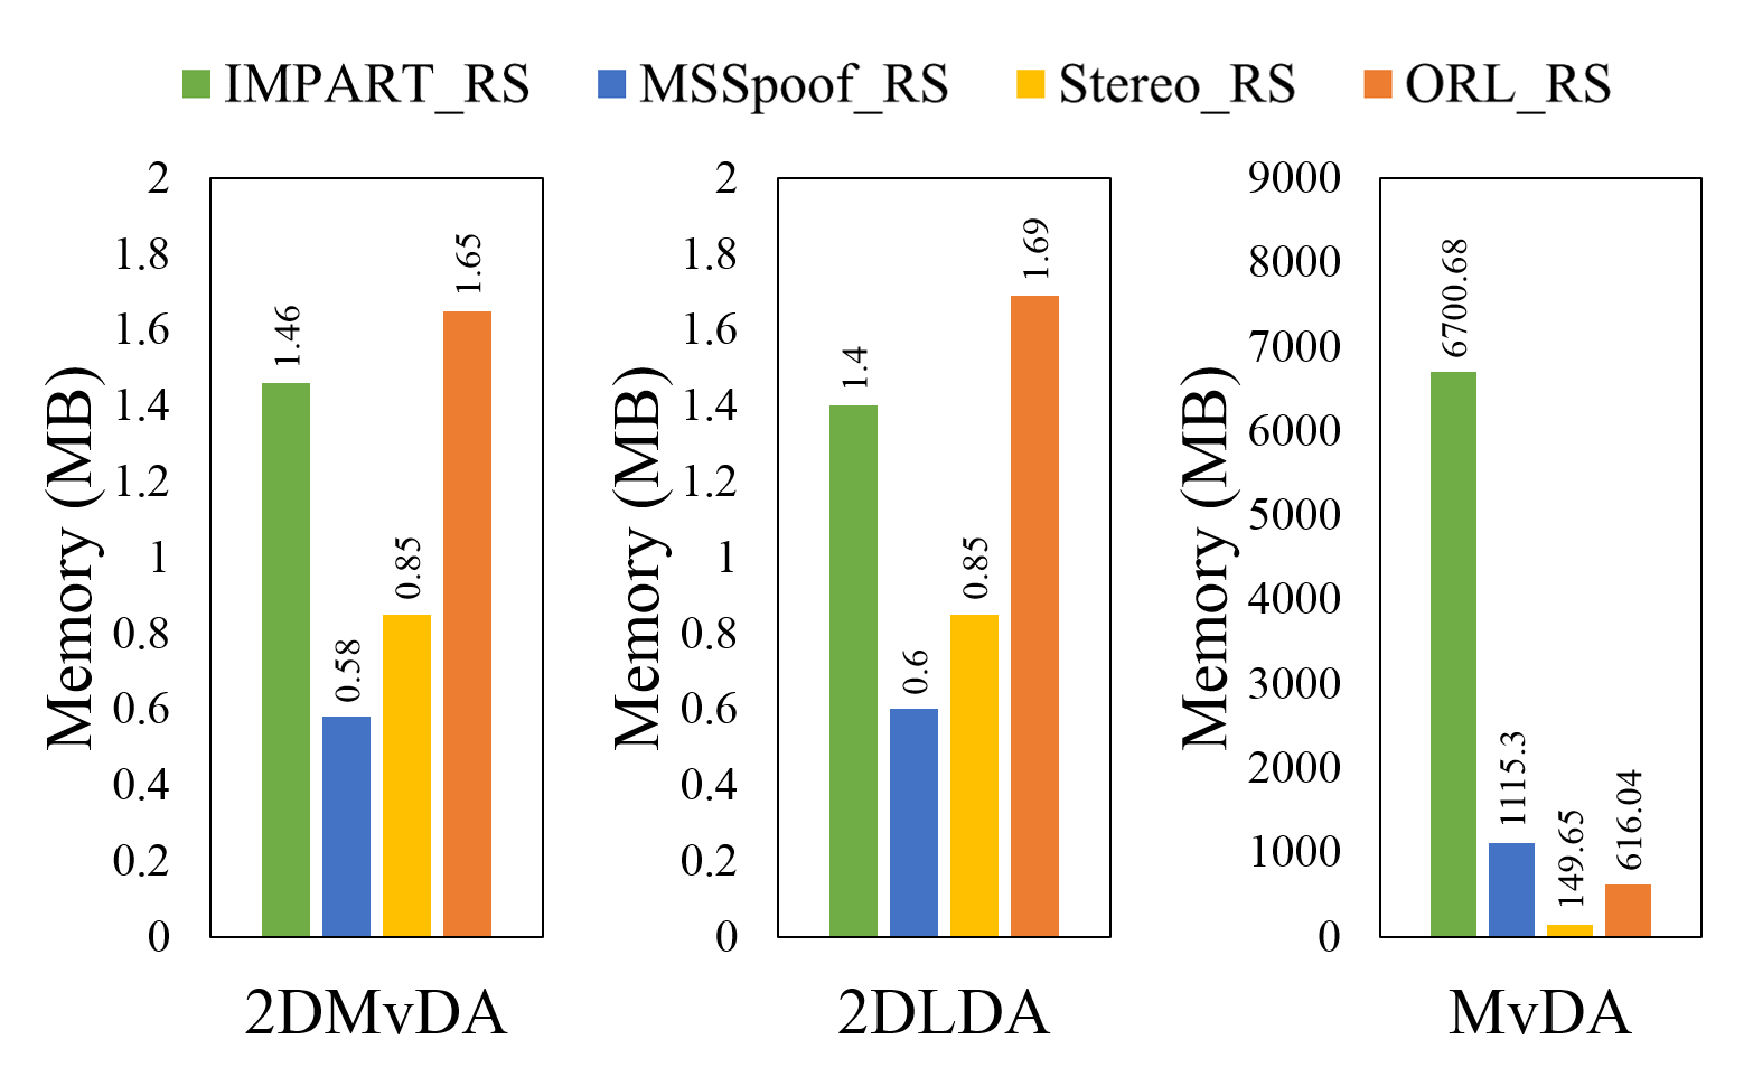
\includegraphics[width=\textwidth]{Figures/2DMvDA/Fig10.pdf}
    \caption{On rescaled datasets}
	\label{fig:2DMvDA_Res_MemoryRS}
  \end{subfigure}
  \begin{subfigure}[h]{0.48\textwidth}
    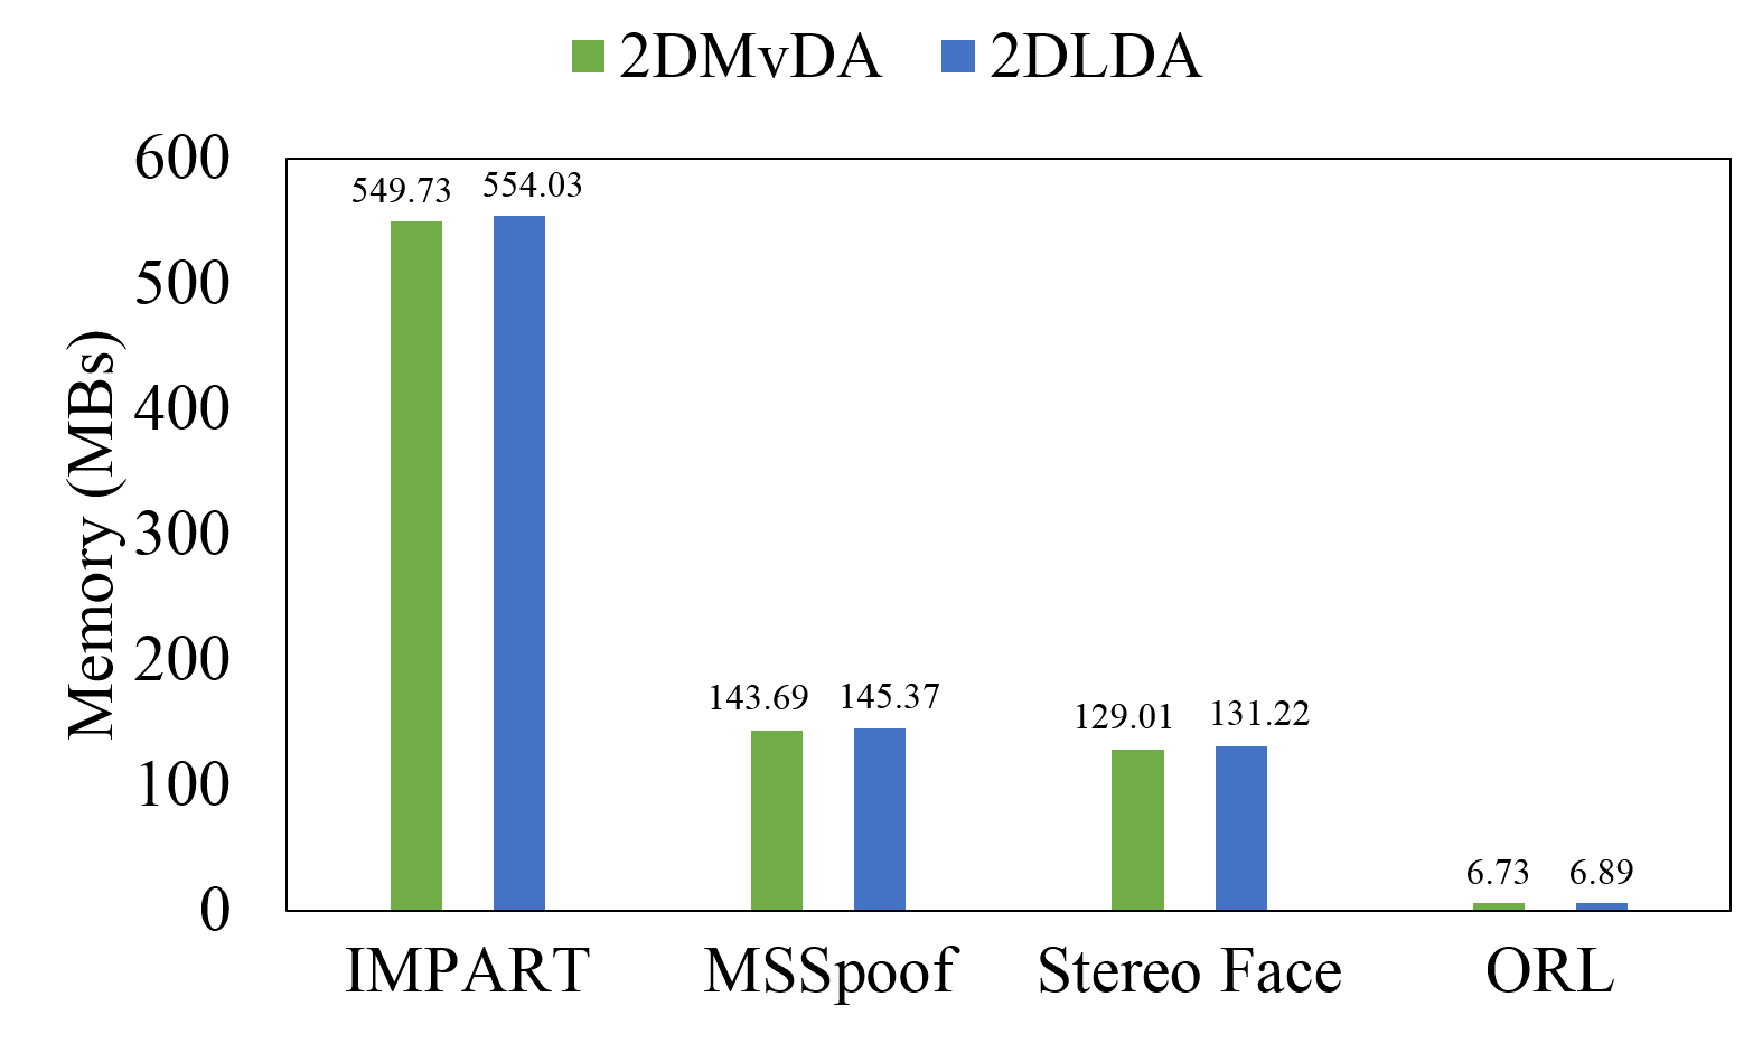
\includegraphics[width=\textwidth]{Figures/2DMvDA/Fig11.pdf}
    \caption{On original datasets}
	\label{fig:2DMvDA_Res_MemoryOrig}
  \end{subfigure}
\caption{Comparison of memory requirement}
\label{fig:2DMvDA_Res_Memory}
\end{figure}

\subsubsection{Memory Usage}
\label{ssubs:2DMvDA_Memory}
\begin{itemize}
\item \textbf{RQ3 :}
Can the use of 2D matrices reduce memory requirements?

\item \textbf{Experiment :}
Record memory usage of (i) all three methods on the rescaled versions of datasets and (ii) 2DMvDA and 2DLDA on the original datasets.

\item \textbf{Discussion :}
The records of memory requirements on the rescaled version of datasets are presented in Fig. \ref{fig:2DMvDA_Res_MemoryRS}. Note that the scale on the y-axis of 2DMvDA and 2DLDA is much smaller than that of MvDA. We see in Fig. \ref{fig:2DMvDA_Res_MemoryRS} that though same as 2DLDA, the proposed method requires less than 0.1\% of the memory required by MvDA to train the model. The difference in memory usage of 2DMvDA against MvDA is due to the latter's need to store large scatter matrices. MvDA uses the vectorized form of images and produces much larger scatter matrices. However, 2DMvDA uses the matrix form, resulting in smaller scatter matrices. This is very advantageous when working with large datasets.

The records of average memory requirements on the original versions of the datasets using 2DMvDA and 2DLDA are presented in Fig. \ref{fig:2DMvDA_Res_MemoryOrig}. We can see that even for original datasets, the 2D methods need less memory than that of MvDA on rescaled datasets. The estimated memory requirement of MvDA for the original version of IMPART dataset is more than 2500 Terabytes, whereas 2DMvDA requires only 0.56 Gigabytes to train on the same dataset. This shows the benefit of using the 2D matrix representation instead of a vectorized form of the image matrix.
\end{itemize}












\section{Summary}
\label{sec:2DMvDA_conc}
The presented classification method, 2DMvDA, is designed for multi-view 2D data. 2DMvDA constructs a common discriminant subspace directly from original 2D matrices, thereby preserving the spatial information in data and eliminating the need for feature extraction in the pre-processing stage.

The proposed method is compared with a 2D single-view method (2DLDA) and a 1D multi-view method (MvDA) for classification accuracy, training time, and memory requirements. 2DMvDA provides better classification results than the other two methods as it benefits from spatial information and multiple views. Even though the gain in classification accuracy is not high, 2DMvDA achieves it with less than 0.01\% of training time and 0.0001\% of memory that MvDA needs to train the same model. 2DMvDA even performs better than 2DLDA with 50\% less training time on average. Also, the comparison of the classification accuracy shows that the proposed method performs better than 2DLDA and MvDA, even with fewer projection dimensions. This work is published in \cite{ShivagundeS22}.

In the next chapter, we present an incremental-decremental method based on 2DMvDA. This method aims to introduce incremental learning in the 2D learning paradigm.

\chapterend
\cleardoublepage